\chapter{Ejercicios y soluciones}



%##############################################################################
%######### ENERO 2023 #########################################################
%##############################################################################

\section*{Enero 2023}
\addcontentsline{toc}{section}{Enero 2023} 
\setcounter{section}{1} % Configura manualmente el contador de secciones


\begin{ejercicio}
	La estrucutra de la figura está formada por átomos de Bi en los nodos de una \fcc, y átomos de Li en todos los huecos octaédricos de dicha \fcc \ de átomos de Bi. El lado de la sc es $a=6.74 \unit{\Angstrom}$. Responde a:
	\begin{enumerate}[label=\alph*)]
		\item ¿Cuál es su forma estequiométrica?
		\item ¿Cuantas ramas de vibración y de qué tipo presenta esta estructura?¿Podrían estar degeneradas para algunas direcciones cristalográficas? En tal caso, explica por qué y pon algún ejemplo (indicando la dirección y las ramas que estarían degeneradas).
		\item Calcula la temperatura de Debye y el calor específico a 300K. Dato: velocidad del sonido en ese material es 1029 m/s. 
	\end{enumerate}
	\begin{center}
		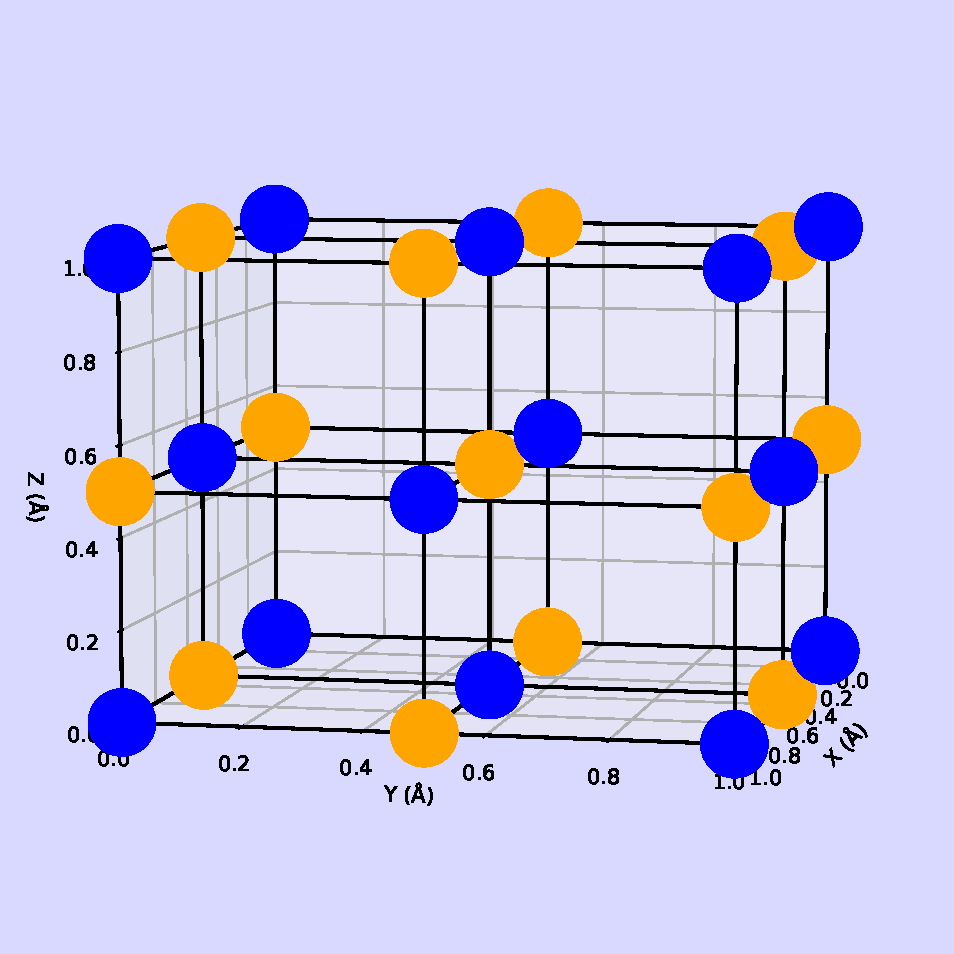
\includegraphics[scale=0.5]{Imagenes/2023-Enero-01.pdf}
	\end{center}
		
\end{ejercicio}	

\begin{ejercicio}
	Sea la red hexagonal simple de la figura ($a=3 \unit{\Angstrom},\ c=4 \unit{\Angstrom}$). 
	\begin{enumerate}[label=\alph*)]
		\item Dibuja sobre la figura unos vectores base e indica las componentes.
		\item Calcula la red recíproca. ¿De qué tipo de red se trata?
		\item Una muestra de polvo con esta estructura se ilumina con RX (rayos X) de longitud de onda $\lambda = 5 \unit{\Angstrom}$. Determina los picos de difracción de menor y mayor ángulo.
		\item Calcula la relación de dispersión electrónica en el marco de la aproximación de electrones fuertemente ligados, utilizando solo orbitales $s$ y teniendo en cuenta hasta segundos vecinos. Calcula las masas efectivas electrónicas $m_x^*,m_y^*$ y $m_z^*$ cerca del fondo de la banda. Datos: $\gamma_1 = 0.4 \ \unit{eV}, \ \gamma_2 = 0.2 \ \unit{eV}$.
		\item Cada átomo aporta un electrón a la conducción, y entre la PZB y la SZB hay un gap de energía despreciable. Indica si el metal es aislante, metal, semimetal o semicondcutor, y que bandas contribuirían a la conducción eléctrica. Justifica las respuestas.
	\end{enumerate}
	\begin{center}
	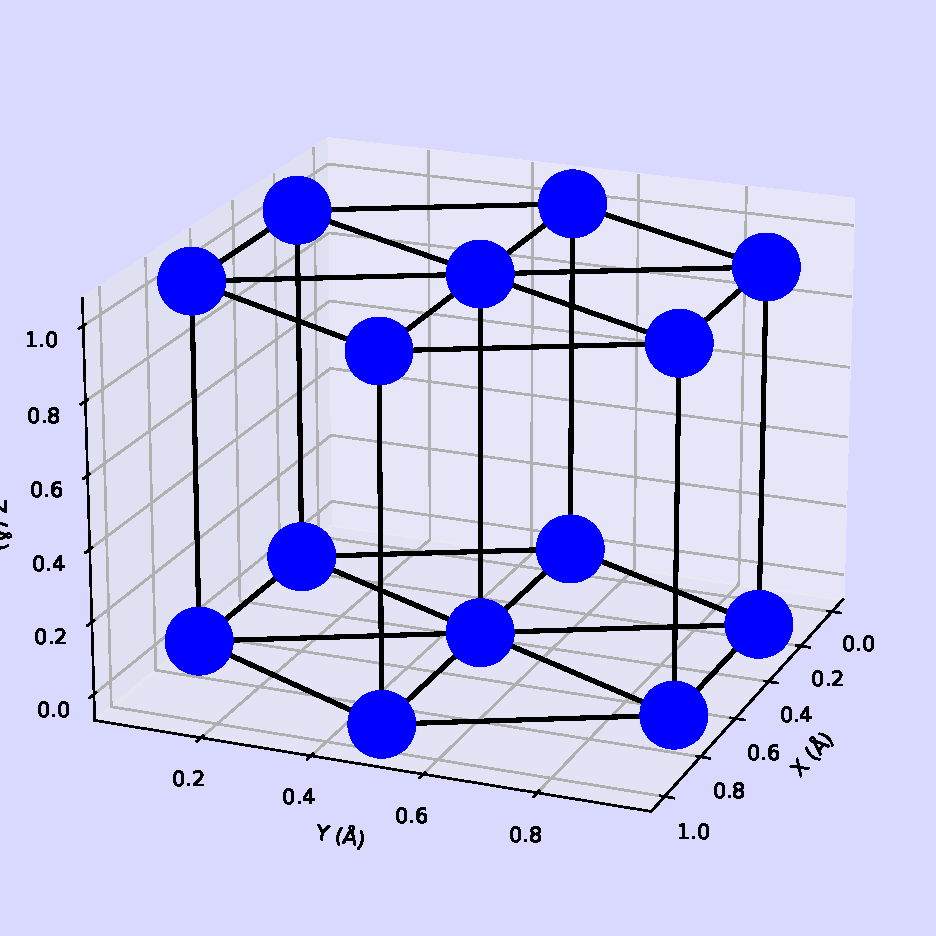
\includegraphics[scale=0.5]{Imagenes/2023-Enero-02.pdf}
	\end{center}
\end{ejercicio}	


\begin{ejercicio}
	Un semiconductor extraído de una computadora tiene como parámetros $\varepsilon_g = 1$ eV, $m_e^* = m_h^* = m_e$. Está dopado con una concentración de aceptores de $N_A = 10^{16} \unit{cm}^{-3}$. Calcular la concentración de electrones y huecos a 300 K. 
\end{ejercicio}	


\begin{solucion}
	\begin{enumerate}[label=\alph*)]
		\item La fórmula estequiométrica es evidente: Li$_3$Bi.
		\item Como sabemos las ramas de vibración dependen de dos factores: la dimensión de la estructura $D$ y el número de átomos dentro de la base atómica $z$. La ecuación es:
		
		\begin{equation}
			\text{Acústicas:} \quad D  \tquad
			\text{Ópticas:} \quad D(z-1)
		\end{equation}
		En nuestro caso $D=3$ y $z=2$. Entonces tenemos 3 ramas acústicas y 9 ramas ópticas, obteniendo los 12 modos normales esperados. La respuesta a la pregunta de si podrían estar degeneradas algunas ramas es complicada, ya que no existe un método unívoco que nos diga cuales son y cuán degeneradas están. Dado la simetría del problema, la respuesta es que en principio deberían estar degeneradas algunas ramas, en particular las vibraciones en las direcciones de las aristas $\hnx,\hny,\hnz$ deberían estar degeneradas. La razón: alta simetría. 
		
		\item La temperatura de Debye viene dada por la ecuación
		\begin{equation*}
			\theta_D= \frac{\hbar \omega_D}{k_B}
		\end{equation*}
		Mientras que la velocidad del sonido $c$ nos permite relacionar $\omega$ Y $k$ tal que $\omega = c k$. Y, como sabemos que $k_D$ viene dada por
		
		\begin{equation*}
			k_D^3 = 6 \pi^2 n
		\end{equation*}
		siendo $n=zN/V$ la densidad numérica de átomos. Entonces podemos obtener $\theta_D$ a partir de los datos dados, ya que $z=4$ y $N/V$ es exactamente igual al número de puntos de red por celda, tal que $N/V=4/a^3$. Entonces:
		
		\begin{equation*}
			\theta_D = \frac{\hbar c}{k_B} \sqrt[3]{6\pi^2 n} \longrightarrow \theta_D = 114.53 \ \text{K}
		\end{equation*}
		La capacidad calorífica a la temperatura $T=300$K. Como $T\approx 2.6 \theta_D$ es válida la aproximación a temperaturas altas en la que:
		
		\begin{equation*}
			C_V=3zNk_B
		\end{equation*}
		 
		Obteniendo como resultado
		\begin{equation*}
			C_V  \approx 25\ \unit{\frac{J}{mol^{-1} K^{-1}}}
		\end{equation*} 
		
	\end{enumerate}
	
\end{solucion}	

\begin{solucion}
	\begin{enumerate}[label=\alph*)]
		\item Los vectores de la base son los siguientes:
		\begin{equation*}
			\an_1 = (a\cdot \sin(30^\circ),a\cdot \cos(30^\circ),0) \tquad 
			\an_2 = (a,0,0) \tquad
			\an_3 = (0,0,c)
		\end{equation*}
		Y en la figura estos vectores son:
		
		\begin{center}
			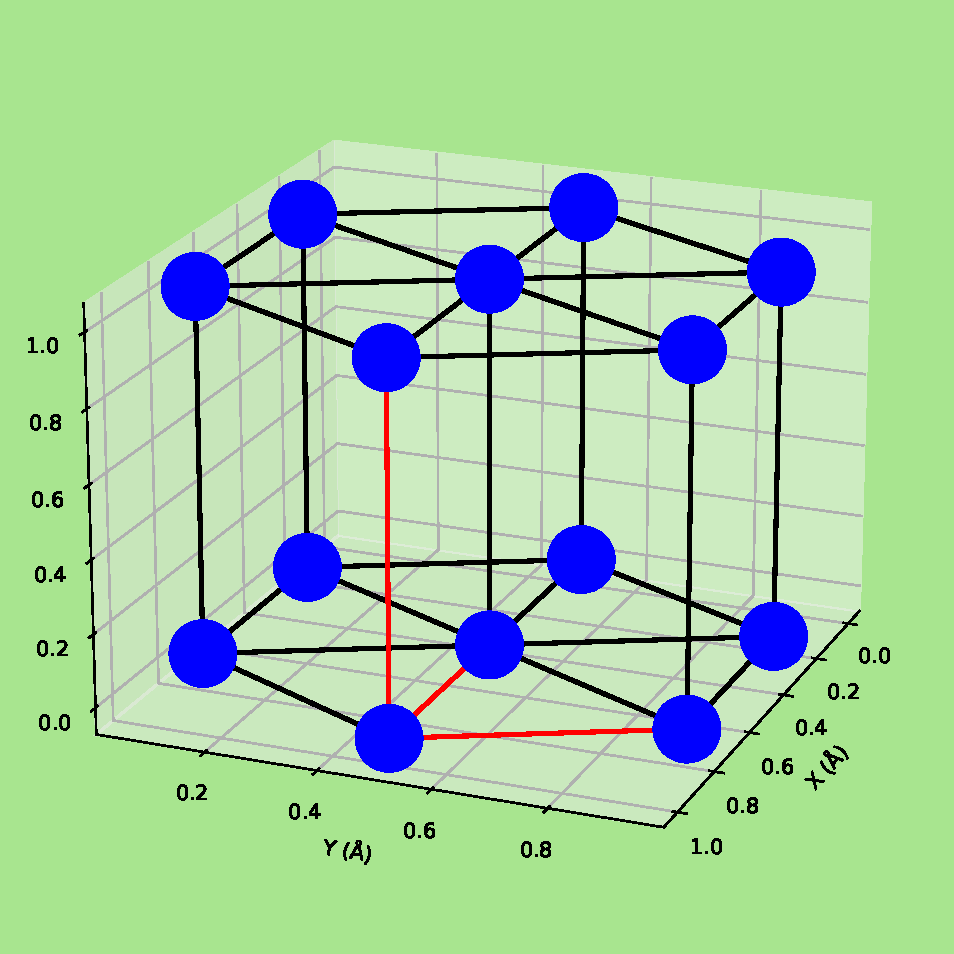
\includegraphics[scale=0.5]{Imagenes/2023-Enero-03.pdf}
		\end{center}
		
		\item Como sabemos la red recíproca viene dada por la siguiente fórmula: 
		
		\begin{equation*}
			\begin{split}    
				\bn_1 & = 2 \pi \frac{\an_2 \times \an_3}{\an_1 (\an_2 \times \an_3)} \\
				\bn_2 & = 2 \pi \frac{\an_3 \times \an_1}{\an_1 (\an_2 \times \an_3)}  \\
				\bn_3 & = 2 \pi \frac{\an_1 \times \an_2}{\an_1 (\an_2 \times \an_3)}
			\end{split} \label{Ec:02-01-04}
		\end{equation*}
		Y por tanto tenemos que la red recíproca de una hexagonal es:
		
		\begin{equation*}
			\bn_1 =  \frac{4 \pi}{\sqrt{3}a} (0,1,0) \quad
			\bn_2 =  \frac{4 \pi}{\sqrt{3}a} (\cos(30^\circ),\sin(30^\circ),0) \quad
			\bn_3 = \frac{2 \pi }{c} (0,0,1)
		\end{equation*}
		Lógicamente existen otras redes válidas en función de los vectores primitivos que cojamos.
		\item Tenemos que obtener los picos de difracción de menor y mayor ángulo. Para esto usamos la ley de Bragg:
		
		\begin{equation*}
			\sin (\theta) = \frac{n\lambda}{2d}
		\end{equation*}
		donde $d=2\pi / |\Gn|$ siendo $\Gn$ un vector cualquiera de la red recíproca. Podemos escribir entonces:
		
		\begin{equation*}
			\sin (\theta) = \frac{n\lambda |\Gn|}{4\pi}
		\end{equation*}
		
		
		 Lógicamente el $\theta$ más pequeño corresponde a $n=1$ y a $|\Gn|_{\min}$. ¿Cual es el $|\Gn|_{\min}$? Pues sería $2\pi/c$. Entonces tenemos que:
		
		\begin{equation}
			\sin (\theta_{\min}) = \frac{\lambda}{2c} \Rightarrow  \theta_{\min} = 38.69^\circ
		\end{equation}
		Para hallar el más grande tenemos que calcular cual es el $n|\Gn|/4\pi$ que se acerca más a 1. Veamos entonces que tenemos que calcular varios. Vamos a probar con varios:
		
		\begin{align*}
			|\Gn|_{[001]} & = \frac{2\pi}{c} = 1.57 \unit{\Angstrom^{-1}} \\ 
			|\Gn|_{[100]} & = \frac{4\pi}{\sqrt{3}a} 2.42\unit{\Angstrom^{-1}}   \\ 
			|\Gn|_{[002]} & = \frac{4\pi}{c} = 3.14 \unit{\Angstrom^{-1}}  \\  
			|\Gn|_{[110]} & = \frac{4 \pi }{\sqrt{3a}} \parentesis{2+\sqrt{3}}^{\sqrt{2}} = 4.17 \unit{\Angstrom^{-1}} \\  
			|\Gn|_{[200]} & = \frac{8 \pi }{\sqrt{3a}} = 4.84 \unit{\Angstrom^{-1}} \\  
		\end{align*} 
		Y como tenemos que $\lambda/4\pi= 0.397 \unit{\Angstrom}$ tenemos que el más grande que da un valor válido $\leq 1$ es $|\Gn|_{[100]}$, de lo que se deduce que el mayor ángulo posible es:
		
		\begin{equation}
			\theta_{\max} = 74.21 ^\circ
		\end{equation}
		
		 \item En primer lugar tenemos que calcular cuantos primeros y segundos vecinos. Dado que $a<c<2a$, tendremos 6 primeros vecinos separados a una distancia de $a$ y 2 segundos vecinos separados a una distancia de $c$. Dado que la aproximación es la de electrones fuertemente ligados tenemos que usar la ecuación:
		 
		 \begin{equation}
		 	\varepsilon(\kn) \approx \varepsilon_s - \beta - \sum_{\Rn} \gamma (\Rn) \cos (\kn \cdot \Rn)
		 \end{equation}
		 Debido a la simetría del problema tendremos que: 
		 
		 \begin{eqnarray*}
			 \varepsilon(\kn) & \approx & \varepsilon_s - \beta -\gamma_1 \left( \cos (k_x a) + \cos \parentesis{ \frac{k_x  a}{2} + \frac{\sqrt{3}}{2} k_y a  } \right. \\  & +  &  \left.    
			 \cos \parentesis{ -\frac{k_x  a}{2} + \frac{\sqrt{3}}{2} k_y a  }+ \cos (-k_x a)	 \right. + \\ & + & \left. \cos \parentesis{ -\frac{k_x  a}{2} - \frac{\sqrt{3}}{2} k_y a  } + \cos \parentesis{ \frac{k_x  a}{2} - \frac{\sqrt{3}}{2} k_y a  } \right)  \\ & - & 2 \gamma_2 \cos (k_z c)   
		 \end{eqnarray*}
		 Lógicamente tenemos que reducir la parte de los cosenos con $\gamma_1$. En primer lugar usamos las propiedades conocidas de $\cos(x)=\cos(-x)$ (el cual ya hemos aplicado para reducir $\gamma_2$) tal que 
		 \begin{eqnarray*}
		 	\varepsilon(\kn) & \approx & \varepsilon_s - \beta -\gamma_1 \left( 2\cos (k_x a) + 2\cos \parentesis{ \frac{k_x  a}{2} + \frac{\sqrt{3}}{2} k_y a  } \right. \\  & +  &  \left.    
		 	2\cos \parentesis{ \frac{k_x  a}{2} - \frac{\sqrt{3}}{2} k_y a  } \right) - 2 \gamma_2 \cos (k_z c)   
		 \end{eqnarray*}
		 Y usando que $\cos (A \pm B) = \cos (A) \cos (B) \mp \sin (A) \sin (B)$ y que $\sin (A\pm B) = \sin (A) \sin(B) \pm \cos(A) \cos(B)$ obtenemos que:
		 
		 \begin{equation*}
		 	\varepsilon(\kn)  \approx  \varepsilon_s - \beta -\gamma_1 2\cos (k_x a) - 4 \gamma_1 \cos \parentesis{ \frac{k_x  a}{2} } \cos \parentesis{ \frac{\sqrt{3}}{2} k_y a  }  - 2 \gamma_2 \cos (k_z c)  
		 \end{equation*}
		 Esta sería la relación de dispersión electrónica teniendo en cuenta hasta segundos vecinos. Las masas efectivas electrónicas son fáciles de calcular, ya que solo tenemos que aplicar la ecuación
		 
		 \begin{equation*}
		 	(m_{ij}^*)^{-1} = \frac{1}{\hbar^2} \eval[\parciales{^2 \varepsilon(\kn)}{k_i \partial k_j}|_{\kn_0}
		 \end{equation*}
		 Veamos que para $m_i^* = m_{ii}^*$ con $i=x,y,z$ las derivadas son:
		 
		 \begin{eqnarray*}
		 	(m_{x}^*)^{-1} & = &  \frac{\gamma_1 a^2}{\hbar^2} \parentesis{2\cos(k_x a) +  \cos \parentesis{ \frac{k_x  a}{2} } \cos \parentesis{ \frac{\sqrt{3}}{2} k_y a  }}
		 	  \\
		 	(m_{y}^*)^{-1} & =  & \frac{3\gamma_1 a^2}{\hbar^2}  \cos \parentesis{ \frac{k_x  a}{2} } \cos \parentesis{ \frac{\sqrt{3}}{2} k_y a  } \\
		 	(m_{z}^*)^{-1} & = & \frac{2 \gamma_2 c}{\hbar^2} \cos (k_z c)
		 \end{eqnarray*}		 
		 Como nos dicen que esto es en el fondo de la banda $\kn\approx 0$, tenemos que
		 
		 \begin{eqnarray*}
		 	(m_{x}^*)^{-1} & = &  \frac{3\gamma_1 a^2}{\hbar^2}	 	\\
		 	(m_{y}^*)^{-1} & =  & \frac{3\gamma_1 a^2}{\hbar^2}   \\
		 	(m_{z}^*)^{-1} & = & \frac{2 \gamma_2 c^2}{\hbar^2}
		 \end{eqnarray*}	
		 Y por tanto las masas son: 
		 
		 \begin{eqnarray*}
		 	(m_{x}^*) & = & \frac{\hbar^2}{3\gamma_1 a^2}= 0.705 m_e	 	\\
		 	(m_{y}^*) & = & \frac{\hbar^2}{3\gamma_1 a^2}=0.705 m_e	  \\
		 	(m_{z}^*) & = & \frac{\hbar^2}{2 \gamma_2 c^2} = 1.191 m_e	 
		 \end{eqnarray*}	
		 \item En este ejercicio uno podría pensar que bastaría decir que tenemos un átomo por celda unidad que aporta un solo electrón, hy que por tanto este siempre será un metal, ya que la banda de valencia estará medio llena siempre, ya que tenemos $2N$ estados posibles de $k$ (el factor 2 es debido al espín) y solo $N$ electrones, de tal forma que la banda de valencia es la única que contiene electrones ergo la única que contribuye a la conducción eléctrica. 
		 
		 Sin embargo, este razonamiento no es el correcto. Cuando tenemos átomos fuertemente ligados hay que tratar con la superficie de Fermi y el volumen de la primera zona de Brillouin. Como sabemos, la primera zona de Brillouin de una red recíproca hexagonal es también un prisma hexagonal.
		 
		 
	\end{enumerate}
\end{solucion}

\begin{solucion}
	Cuando dopamos un semiconductor tenemos dos posibilidades en función de $T$: que el número de impurezas sea irrelevante en comparación a las fluctuaciones térmicas y que por tanto podamos asumir que estamos en el régimen intrínseco ($n=p$), o que estemos en un régimen extrínseco en el que se verifique $N_A=p$ o $N_D=n$. La estimación de la temperatura $T_i$ es sencilla, hacemos que $n\approx N_A \rightarrow p \approx 2N_A$
	
	\begin{equation}
		2N_A^2 = N_c N_v e^{-\varepsilon_g / k_B T_i}
	\end{equation}
	Tal que:
	\begin{equation}
		T_i = \frac{\varepsilon_g}{k_B} \frac{1}{\ln (2N_A^2 / N_c N_v)}
	\end{equation}
	Usando que $N_c = N_v = 2.5 \times 10^{19} \ \unit{cm^{-3}}$ en nuestro caso (sustituimos en la ecuación general $N_c(T)$ la temperatura $T=300$K cuando estamos en el régimen no degenerado, el cual se verifica si $\varepsilon_g \gg k_B T$, como en nuestro caso), tenemos que:
	
	\begin{equation}
		T_i = 776 \ \unit{K}
	\end{equation}
	Como estamos en el caso extrínseco podemos hacer que $p=N_A$ y por tanto solo resta calcular $n$ que se hace a partir de:
	
	\begin{equation}
		n p = N_c N_v e^{-\varepsilon_g / k_B T}
	\end{equation}
	De lo que deducimos 
	
	\begin{equation}
		n  =  \frac{N_c N_v}{N_A} e^{-\varepsilon_g / k_B T}
	\end{equation}
	obteniendo que:
	
	\begin{equation}
		p = 10^{16} \ \unit{cm^{-3}} \tquad n = 6.14 \times 10^6 \ \unit{cm^{-3}}
	\end{equation}
	
\end{solucion}	


\newpage

%##############################################################################
%######### ENERO 2021 #########################################################
%##############################################################################

\section*{Enero 2021}
\addcontentsline{toc}{section}{Enero 2021} 
\setcounter{section}{2} % Configura manualmente el contador de secciones

\begin{ejercicio}
	El dibujo representa la celda primitiva de un superconductor de alta temperatura crítica muy estudiado. Los ángulos entre los ejes $a,b,c$ son rectos. Indica el tipo de red cristalina, rodea con un círculo los átomos de una posible base atómica y escribe la fórmula estequiométrica. 
	
	\begin{center}
		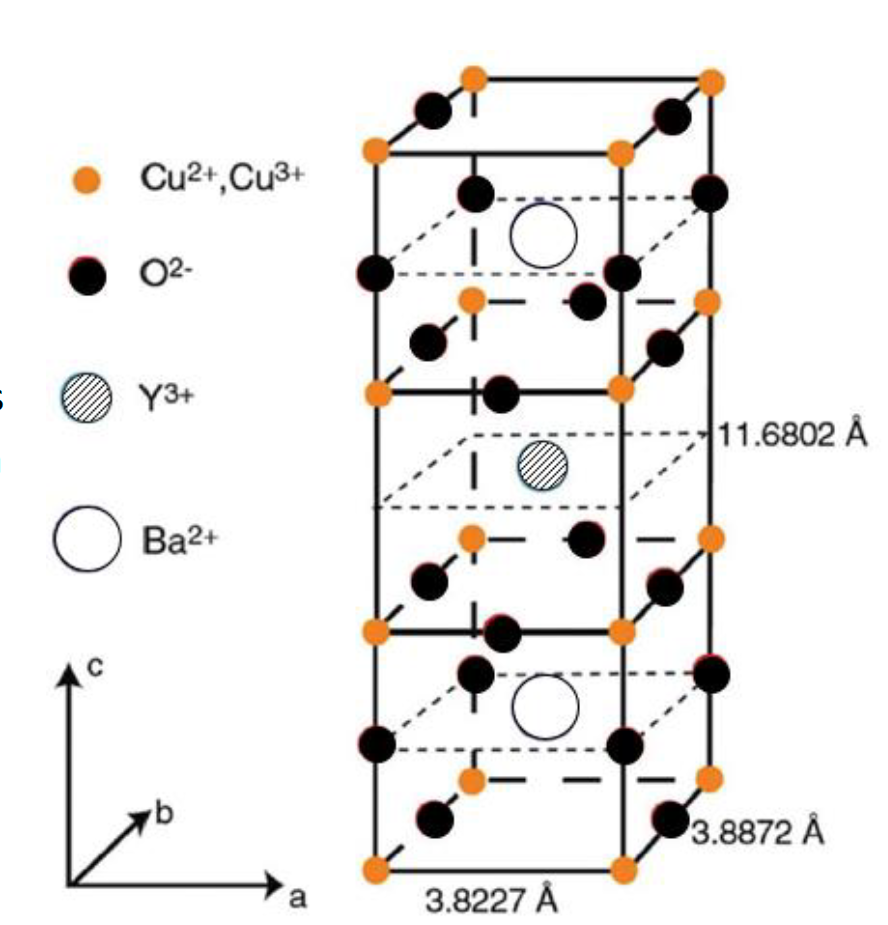
\includegraphics[width=0.4\textwidth]{Imagenes/Enero_2021_01.png}
	\end{center}
	
	
	
\end{ejercicio}

\begin{ejercicio}
	Explica en qué consiste la aproximación de Debye, para qué se utiliza, y qué sentido físico tienen la frecuencia de Debye y la temperatura de Debye.
\end{ejercicio}

\begin{ejercicio}
	Un sólido cristalino monoatómico tiene una estructura de la que se duda entre cúbica simple y tetragonal simple. Para determinarla se le somete a un difractómetro de rayos X en polvo cuyo difractograma obtenido es como se muestra. Analizando los máximos, argumentar si el difractograma es compatible con alguna de las dos estructuras.
	
	\begin{center}
		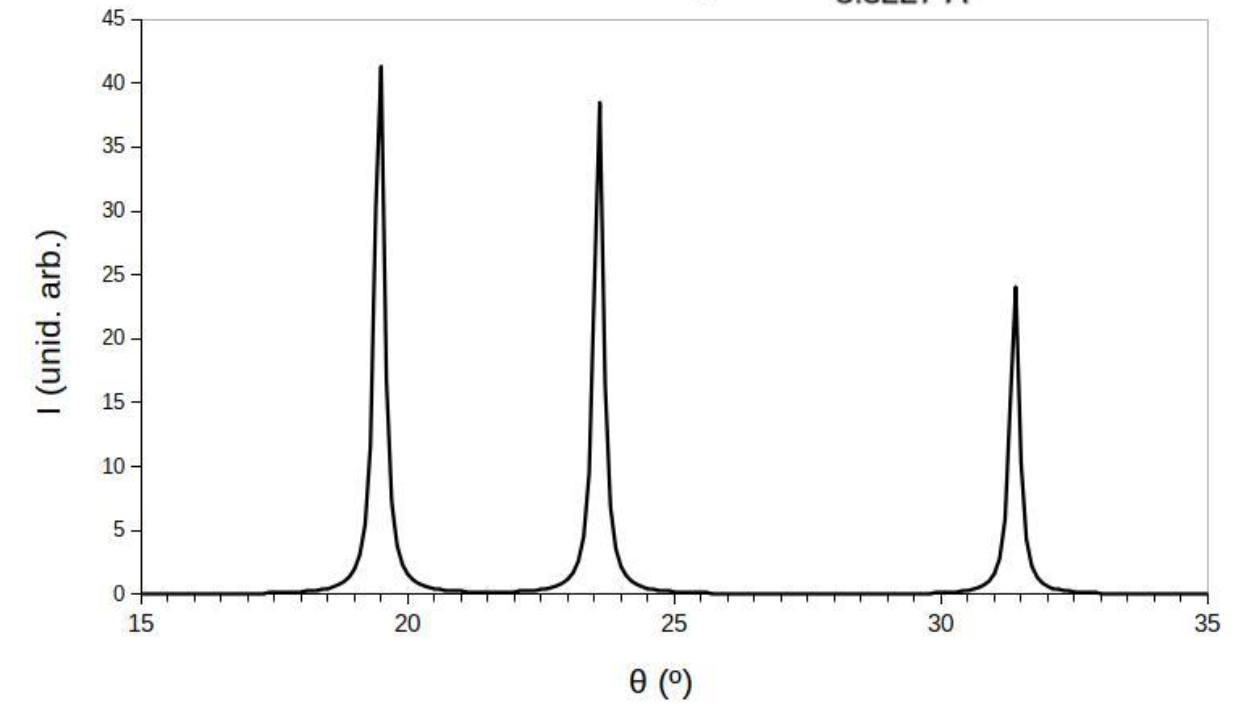
\includegraphics[width=0.4\textwidth]{Imagenes/Enero_2021_02.png}
	\end{center}
	
\end{ejercicio}

\begin{ejercicio}
	Sea un gas de Fermi de electrones libres en el que cada estado $k$ está ocupado con un solo electrón con espín $\uparrow$ (en teoría esta situación podría conseguirse aplicando un campo magnético suficientemente alto). Calcula el aumento de energía cinética respecto al estado fundamental (en el que hay dos electrones por estado $k$).
\end{ejercicio}

\begin{ejercicio}
	Sea una estructura \bcc \ monoatómica con parámetro de red (de la celda cúbica) $a=$0.5 nm. 
	\begin{enumerate}[label=\alph*)]
		\item Determinan el mayor y menor vector de onda posible de sus modos normales de vibración. ¿Cambiaría la respuesta si existiera una base atómica de más de un átomo?
		\item Los átomos que forman la estructura son divalentes, y el potencial periódico que ejercen sobre los electrones crea un gap de energía de 1.5 eV sobre la frontera de la primera zona de Brilluoin. Suponiendo que la estructura electrónica puede describirse por la aproximación de electrones cuasilibres, discute si el material es aislante, metálico, semimetálico o semiconductor.
		
	\end{enumerate}
	
	\begin{center}
		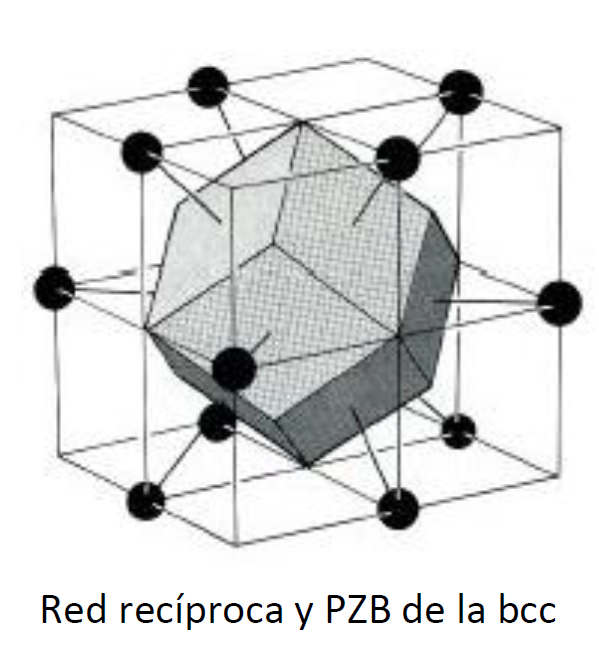
\includegraphics[width=0.4\textwidth]{Imagenes/Enero_2021_03.png}
	\end{center}
	
\end{ejercicio}

\begin{ejercicio}
	¿Se puede decir algo seguro sober la capacidad de conducir sobre la capacidad de conducir de un hipotético metal de valencia impar con un número impar de átomos por celda primitiva?
\end{ejercicio}

\newpage

%##############################################################################
%######### ENERO 2020 #########################################################
%##############################################################################

\section*{Enero 2020}
\addcontentsline{toc}{section}{Enero 2020} 
\setcounter{section}{3} % Configura manualmente el contador de secciones

\begin{ejercicio}
	Sea la estructura hexagonal compacta (\hcp) de átomos monovalentes de la figura. La separación entre vecinos próximas es $a=1\unit{\Angstrom}$. La figura inferior representa su PZB.
	\begin{enumerate}[label=\alph*)]
		\item Calcula el valor que tendría el vector de Fermi según el modelo de electrones libres.
		\item Calcula el factor de estrucutar de la base $S_\Gn$. Comprueba que $S_\Gn=0$ para los $\Gn$ asociados a las caras hexagonales de la PZB (eso conllevaría la anulación de un posible gap de energía sobre esas caras).
		\item En el marco del modelo de electrones cuasilibres, explica si a $T=0$ K el material sería conductor, aislante o semimetal.
		\item Indica el grado de degeneración de los estados $L,H,K$ y $A$ de la figura.
	\end{enumerate}
\end{ejercicio}

\begin{ejercicio}
	En una estructura \fcc monoatómica con $a=0.3$ nm, un difractograma en polvo, usando que $\lambda=0.1$ nm, tiene uno de los máximos en $\theta=19.47^\circ$. ¿A qué ángulo aparecerá el siguiente pico?
\end{ejercicio}

\begin{ejercicio}
	¿Cómo cambiaría la separación entre vecinos próximas y la energía de cohesión del $\ce{Ce^- Na^+}$ si los iones tuviesen el doble de carga?
\end{ejercicio}

\begin{ejercicio}
	¿El número de colisiones $U$ entre fonones (que son las que disminuyen la conductividad térmica reticular $\kappa_{\text{ret}}$) crece siempre con la temperatura $T$?¿Es eso compatible con que $\kappa_{\text{ret}}$ crece con $T$ a bajas temperaturas?
\end{ejercicio}

\begin{ejercicio}
	Consideremos la dilatación térmica de un metal. ¿Cómo es afectada la energía (cinética) total de los electrones de conducción?¿Aumenta o disminuye? Argumenta.
\end{ejercicio}

\begin{ejercicio}
	Utilizando el método de electrones fuertemente ligados calcula $\varepsilon(\kn)$ para una estructura cúbica simple (utiliza la aproximación de orbitales $s$). A partir del resultado calcula las masas efectiva cerca del fondo de la banda. ¿Cómo son en esa región las superficies de energía constante?
\end{ejercicio}
\begin{ejercicio}
	Para un semiconductor dopado con impurezas aceptoras, representa gráficamente la concentración tanto de huecos como de electrones frente a la temperatura. Utiliza la representación de Arrhenius: $\log (n,p) $ vs $1/T$.
\end{ejercicio}

\begin{ejercicio}
	Representa (y justifica) el comportamiento de la magnetización frente a $B/T$ de un material paramagnético. A temperatura ambiente: ¿de qué orden es el campo magnético que haría falta para alinear los momentos magnéticos atómicos?
\end{ejercicio}

\newpage


\section*{Julio 2019}
\addcontentsline{toc}{section}{Julio 2019} 
\setcounter{section}{4} % Configura manualmente el contador de secciones

\newpage

\section*{Enero 2019}
\addcontentsline{toc}{section}{Enero 2019} 
\setcounter{section}{5} % Configura manualmente el contador de secciones


